\documentclass[12pt]{article}
\usepackage{graphicx}
\usepackage{epsfig,color,amsmath}
\usepackage{varioref}
\usepackage{ae,aecompl}
\usepackage[dvipdf,ps2pdf,hyperfigures,bookmarks]{hyperref}

\setcounter{topnumber}{6}
\setcounter{bottomnumber}{6}
\setcounter{totalnumber}{6}

\setcounter{secnumdepth}{-1}
\setcounter{tocdepth}{5}

\addtolength{\topmargin}{-1.5truecm}
\addtolength{\textheight}{3.0truecm}
\addtolength{\textwidth}{2truecm}
\addtolength{\oddsidemargin}{-1.5truecm}
\addtolength{\evensidemargin}{-1.5truecm}

\renewcommand{\floatpagefraction}{1.0}      %  allows big pictures
\renewcommand{\dblfloatpagefraction}{1.0}
\renewcommand{\topfraction}{1.0}
\renewcommand{\textfraction}{0.0}           % minimum text fraction
\renewcommand{\bottomfraction}{1.0}

\parindent0pt
\parskip3pt

\definecolor{mygrey}{rgb}{0.4,0.4,0.4}
\definecolor{mygreen}{rgb}{0.0,0.5,0.0}

\begin{document}

\fontfamily{phv}
\fontseries{m}
\selectfont
\renewcommand{\rmdefault}{phv}

{\color{red} \begin{center} This Handbook is partially out of date! \end{center} }
\tableofcontents

\clearpage

\begin{center}
{\huge \bf Simulator Handbook}
\end{center}

\section{Introduction}

With this neural net simulator, you edit your own network and training algorithm using a built-in ``batch''-language.
In this language, you specify every detail of your algorithm.
You may extend the language by adding and compiling to the simulator your own functions written in C.
The language is pre-structured to work itself down
from {\sl iterations} to {\sl relaxations (over time)} to {\sl area (layer) visits} to {\sl neuron visits}.
A variety of networks with connectionist neurons can be programmed with ease, in particular if neuronal updates are local.
Examples are: Hopfield networks, Boltzmann- and Helmholtz machines, backpropagation-trained multi-layer perceptrons.
Non-local interactions can also be implemented (like winner-finding within one layer of a Kohonen network)
but severely non-local operations (like matrix inversion for standard ICA) will make you program your whole algorithm in a C-procedure.

 \begin{figure}[htb]
 \begin{center}
 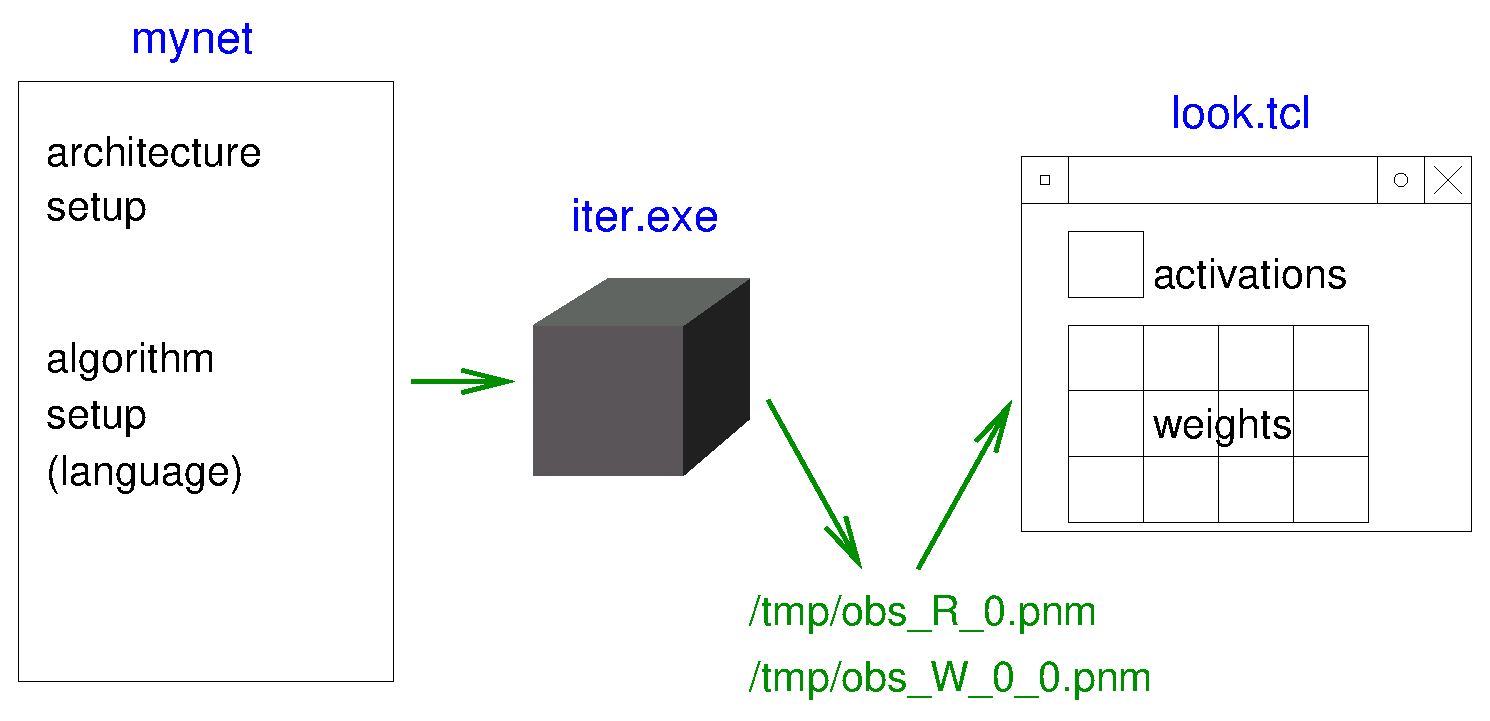
\psfig{file=figs/informationflow.eps,width=12cm}
 \end{center}
 \vspace*{-7mm}
 \caption{Information flow: language file ${\color{mygreen}\rightarrow}$ code ${\color{mygreen}\rightarrow}$ image files ${\color{mygreen}\rightarrow}$ display tool.}
 \label{informationflow}
 \end{figure}

The activations as well as the neuronal weights (synaptic strengths) shall be written periodically into the \texttt{/tmp/coco/} directory of your computer as image files.
Then a separate, non-interactive GUI ``\texttt{look.tcl}'' will collect and display these results.


\vspace*{-6mm}
\section{Installation}

\vspace*{-4mm}
The simulator has been tested on a couple of UNIX/Linux systems and on Windows with cygwin.
It requires something equivalent to
{\sl (i)} \texttt{g++} for compilation,
{\sl (ii)} \texttt{lex} and \texttt{yacc} to generate the parser of the language file and
{\sl (iii)} \texttt{Tcl/Tk} for the result viewer \texttt{look.tcl}.
Get the file \texttt{coco06.tar}.
Then type \texttt{tar xvf coco06.tar} which creates the subdirectory \texttt{coco06/} with the simulator in it.
Type \texttt{./make} in \texttt{coco06/} which creates the executable \texttt{cococo} (and also \texttt{prae.exe} as a pre-processor).



\subsection{Directories and files}

This structure is currently undergoing frequent changes. Don't take serious!

\begin{tabular}{ll}
\underline{coco06/}       & main directory \\
{\color{blue}cococo}      & the executable \\
{\color{blue}look.tcl}    & ``GUI'' (image viewer) \\
prae.exe                  & called by \texttt{cococo}, praeprocesses the language file \\
make                      & only for convenience here \\[6pt]

\underline{d/}            & data used for training \\[6pt]

\underline{src/kernel/}   & C source files \\
Makefile                  & type \texttt{make} to compile the program \\
series.h                  & typedef struct's: \texttt{SIMULATION SERIES SWEEP STAY COMMAND} \\
coco.h                    & typedef struct's: \texttt{STATE AREA AGENT PARAMS DATA} \\[6pt]

coco.c                    & \texttt{main()}, calls \texttt{do\_simulation} \\
relax.c ~.h               & \texttt{do\_simulation} does nested loops: series - sweep - stay - command \\
vehicle.c ~.h             & memory allocation, initialization, function assignments \\[6pt]

local.c ~.h               & functions for local computations on neurons \\

utils.c ~.h               & e.g. for matrix memory allocation \\[6pt]

\underline{src/parser/}   & parser directory for the language \\
 Makefile                 & called by \texttt{src/Makefile}, this makes \texttt{prae.exe} \\
 prae.c                   & praeprocesses the language file \\
 r.lex                    & definitions of lexical elements \\
 r.yacc.c, ~.h            & grammar definition (also allocates \texttt{SIMULATION AGENT PARAMS}) \\[6pt]

\underline{v/}            & network description files (language) \\
{\color{blue}mylanguagefile} & edit your own file! \\[6pt]

\underline{docu/}         & e.g. handbook.ps \\[6pt]

\underline{/tmp/coco/}    & activations and weights as \texttt{pnm}-image files \\

\end{tabular}


\section{Program call}

In general, start the program in \texttt{coco04/} with the following call:\\
\hspace*{11mm} \texttt{./cococo -file v/mylanguagefile} \\
This will start the program with it reading the language file \texttt{v/mylanguagefile}.
The program will allocate memory for the network you defined,
it will run the activation \& training algorithm over and over again, as you have described in your language file.
Make sure a directory for the activations \& weights exists (e.g. \texttt{/tmp/coco/}).

\subsection{Options}
\begin{tabular}{p{3.7cm}p{11.3cm}}
\texttt{-analyze 1}        & The weights will {\bf not} be exported/overwritten into files.\\
\texttt{-seed n}           & Initializes the random seed to number \texttt{n}.\\
\texttt{-set string value} & Fill-in the macro which appears as \texttt{\$string} in the language file with \texttt{value}.
                             This option invites you to write a shell script
                             which calls the simulator with different parameters over and over again.
\end{tabular}

\subsection{``GUI'' (image file viewer)} After starting the program, start from a separate shell the file viewer like:\\
\hspace*{11mm} \texttt{./look.tcl a w 0 1}\\
where ``\texttt{a}'' means display activation files,
``\texttt{w}'' means display weight and threshold files,
and numbers ``\texttt{n}'' specify the areas from which to collect these files.
In the window, click the left mouse button or Return to reload the files, right mouse button to quit.

The program \texttt{cococo} writes the activations to be observed and all weights and thresholds into the directory \texttt{/tmp/coco/} (this directory is actually set in the language file, and is a variable in the file \text{look.tcl}).
The file names are composed of
{\sl (i)} the beginning ``\texttt{obs\_}'',
{\sl (ii)} the activation or weight name (a letter), or ``\texttt{Th}'' for thresholds,
           followed via underscore ``\texttt{\_}'' by the area number(s) involved and
{\sl (iii)} the ending ``\texttt{.pnm}''.
For example, weights $W$ from area \texttt{0} to area \texttt{1} are called ``\texttt{obs\_W\_1\_0.pnm}''.
This image file can also be used to import the weights, but a file ``\texttt{obs\_W\_1\_0.ext}'' with higher resolution for the weight values will actually be used.
The image viewer will display below the image files their truncated names as well as the minimum and maximum values.

If you want to change the sizes for display, you can change the zoom-factor in the tcl-script file \texttt{look.tcl}.
Search for the expression ``zoom'' within \texttt{look.tcl} and change the number behind (must be an integer).

If you want the files to be reloaded and displayed continually, switch to auto-update by editing \texttt{look.tcl}:
change the initialization of the variable, \texttt{set AUTOREFRESH 0} , to: \texttt{set AUTOREFRESH 1}.


\section{The language}

A language file has three main parts, describing {\sl (i)} global variables, {\sl (ii)} area sizes and {\sl (iii)} the algorithm.

\subsection{Global variables}

Here you define first three specific global variables
and then introduce an arbitrary number of own standardized pointers to memory space.

\texttt{global \{} \\
\begin{tabular}{p{2.25cm}p{12.75cm}}
\texttt{iter} &
  is the time at which the simulation starts, usually 0.
  {\color{red} Setting might be ignored here!} \\
\end{tabular}
\begin{tabular}{p{2.25cm}p{12.75cm}}
\texttt{areas} &
  is the number of areas. For example, ``\texttt{2}'' will create areas \texttt{0} and \texttt{1}.\\
\end{tabular}
\begin{tabular}{p{2.25cm}p{12.75cm}}
\texttt{mult} &
  is the multiplicity of activation values. Use ``\texttt{1}'' here, since more aren't supported by any functions yet.\\
\end{tabular}

\begin{tabular}{p{2.25cm}p{12.75cm}}
\texttt{ptr1 " "} &
  here some standardized pointers to memory space are introduced, to be used in the algorithm by their name (e.g. \texttt{ptr1}).
  Pointers have a void \texttt{data} pointer entry and a string which can be set here.
  They can be useful here to set directories or files for data import or export.\\
\end{tabular}
\texttt{\}}


\subsection{Area sizes}

The part introduced by ``\texttt{all}'' defines the areas' default sizes (areas are rectangular):

\texttt{all \{} \\
\begin{tabular}{p{2.25cm}p{12.75cm}}
\texttt{d\_a} &
  is the vertically displayed size, indexed by the slow counting index.\\
\end{tabular}
\begin{tabular}{p{2.25cm}p{12.75cm}}
\texttt{d\_b} &
  is the horizontally displayed size, indexed by the fast counting index.\\
\end{tabular}
\texttt{\}}

Individual properties of specific areas, for example for area \texttt{0} may be specified, e.g.:

\texttt{area 0 \{} \\
\begin{tabular}{p{2.25cm}p{12.75cm}}
\texttt{d\_b} &
Only those properties that differ from the defaults need to be specified,
but don't leave this list empty (may cause syntax problems)!
\end{tabular}
\texttt{\}}


\subsection{Algorithm}

Structures contain all information about the algorithm in 4 nested levels.
From the outside to the inside, we find first ``\texttt{series}'', ``\texttt{sweeps}'' and ``\texttt{stays}'' which are concerned with repetitions, time-, area- and neuron selection.
The inner level, ``\texttt{commands}'', does essentials like taking data, computing neuronal activations or doing the learning.

\begin{enumerate}
\item ``series'' repeat over and over again, e.g.\ for each time picking up a new data point.
      The syntax to repeat {\color{blue} ilen} times is:\\[6pt]
      \texttt{series (} {\color{blue} ilen} \texttt{) \{} \\
      \texttt{\}}

\item ``sweeps'' relaxate in time, i.e.\ with the one data point, update the neurons possibly a couple of times.
      The syntax to iterate (relaxate) from time {\color{blue} begin} to time {\color{blue} end} while visiting the areas (``stays'') in the {\color{blue} area\_order} given. is:\\[6pt]
      \texttt{sw (} {\color{blue} begin} {\bf ;} {\color{blue} end} {\bf ;} {\color{blue} area\_order} \texttt{) \{} \\
      \texttt{\}}

\item ``stays'' visit a given area. The syntax to visit neurons on area no.\ {\color{blue} area} in the {\color{blue} neuron\_order} given is:\\[6pt]
      {\color{blue} area} \texttt{(} {\color{blue} neuron\_order} \texttt{)}

\item ``commands'' compute a ``target'' value on a neuron, using a selected ``function'', ``source area(s)'', ``source value(s)'' and optional parameters.
      The syntax is:\\[6pt]
      \texttt{\{} {\color{blue} target} {\bf ;} {\color{blue} function} {\bf ;} {\color{blue} source area(s)} {\bf ;}
      {\color{blue} source value(s)} {\bf ;} {\color{blue} parameters} \texttt{\}}
\end{enumerate}

Note that since \texttt{stays} are nested within \texttt{sweeps},
first all areas within a \texttt{sweep} are visited at relaxation time 0, and only then all areas at time 1 and so on.

{\footnotesize
Find out more about these structures in the header file \texttt{series.h}.
Starting from the back, you will find that each outer structure has (a) pointer(s) to its ``nextmost'' inner structure
as well as an \texttt{int}eger telling how many of those inner structures are contained.
From outside to the inside we have the structures:
\texttt{SIMULATION}, \texttt{SERIES}, \texttt{SWEEP}, \texttt{STAY}, \texttt{COMMAND}.
The outermost, \texttt{SIMULATION} structure is a cover to allow for several \texttt{SERIES}, but it is not reflected in the language.

Find out more about the use of these structures in the program file \texttt{relax.c}.
There, from the outermost to the innermost (in \texttt{relax.c} from back to front),
each structure is worked over to work over the structures contained within.
The functions are: \texttt{do\_simulation}, \texttt{do\_series}, \texttt{do\_sweep}, \texttt{do\_stay}, \texttt{do\_command}.
}

The {\color{blue} area\_order} argument of a \texttt{sweep} is usually \underline{``\texttt{order}''} so that \texttt{stays} are selected in order.
The arguments \underline{``random''} or \underline{``propto''} choose the \texttt{stays} randomly.
We need this only for a Glauber dynamics in an attractor network with several layers (see \texttt{relax.c} if you want to use these).

The {\color{blue} neuron\_order} argument of a \texttt{stay} is usually
\underline{``\texttt{o}''} to select the neurons in order,
\underline{``\texttt{r}''} to select them randomly or
\underline{``\texttt{s}''} to shuffle, i.e.\ to select them randomly in a way that each comes once.
Here, a command is done locally on one neuron.

The {\color{blue} neuron\_order} parameter \underline{``t''} (for total) of a \texttt{stay}, however, determines that a command is only done once on a whole area.
This is appropriate for some functions, e.g. a non-local function to find the maximum-active neuron.
Its use therefore implies the use of an appropriate function in the respective \texttt{command}.

The {\color{blue} area\_order} parameter \underline{``alltime''} of a \texttt{sweep} even determines that a command is done only once on an area for a whole \texttt{sweep},
i.e. at all time steps of that relaxation and, of course, for all neurons in the respective areas.
Appropriate functions then have to be used in all commands under that \texttt{sweep}.
This is convenient for functions that assign training data to the neural activations or for functions to export the activations for display.
The relaxation duration parameters {\color{blue} begin} and {\color{blue} end} are internally passed on as parameters,
and the \texttt{neuron\_order} parameters of the \texttt{stays} are ignored here.

 \begin{figure}[htb]
 \begin{center}
 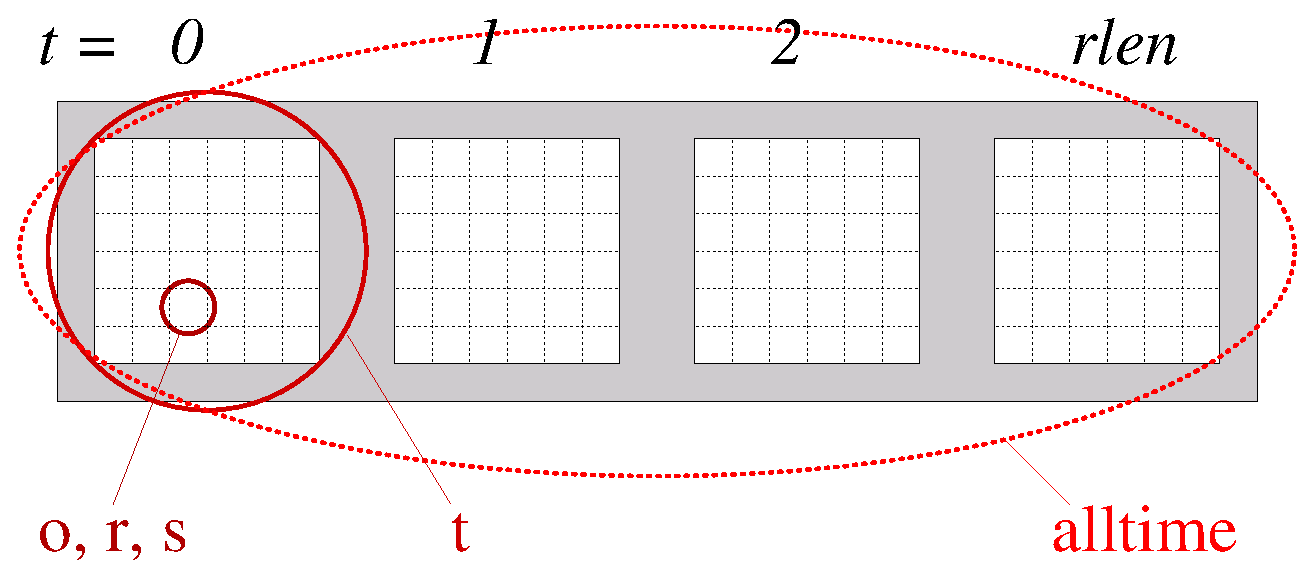
\psfig{file=figs/functionscope.eps,width=9cm}
 \end{center}
 \caption{Function Scopes.
          Each of the 4 larger squares shows the neurons of one square area at one relaxation time step, in the way it is also displayed in the GUI look.tcl.
          4 relaxation steps are performed, from $t = 0$ to $t = rlen$.
          The circles denote one invocation of the corresponding command function:
          if the \texttt{stay}'s {\color{blue} neuron\_order} argument is ``\texttt{o}'', ``\texttt{r}'' or ``\texttt{s}'', then the function is executed for every neuron.
          If it is ``\texttt{t}'', the function will be executed only once for an area.
          If the \texttt{sweep}'s {\color{blue} area\_order} argument is \texttt{alltime}, then the command function is invoked only once during a whole relaxation.
          }
 \label{functionscope}
 \end{figure}

\paragraph{Commands} $\,\!$
Only the {\color{blue} target}s are updated within a command.
Every \texttt{command} has a neural activation as target which is denoted by a capital letter from \texttt{A} to \texttt{Z}.
Additionally, after a ``\texttt{\bf ,}'' (comma), a standardized pointer, or several separated by a  ``{\bf \texttt{+}}'' symbol may be used, e.g. for weights.
The pointers allow read and write access by the command function
and they may have been introduced already in the \texttt{global} section of the language file in which case their string argument is already initialized.

The {\color{blue} function} is what computes the target. Its string name is similar to the C-procedure name.
Function keys in the C-program denote whether a function is used for 's'=single (``o'', ``r'' or ``s'') neuron update, for 't'=total area update or invoked in a 'a'=alltime manner.
For sloppy use, 'v'=versatile (total or alltime) or 'n'=nevermind (single or total or alltime) are also supported.

{\color{blue} Source areas} are denoted by the area numbers from which to take the {\color{blue} source values} which are activations (letters from \texttt{A} to \texttt{Z}).
Several {\color{blue} source areas} can be separated by a ``{\bf \texttt{,}}'' or by a ``{\bf \texttt{+}}'',
and the same structure of ``{\bf \texttt{,}}'' and ``{\bf \texttt{+}}'' must then be reflected in the {\color{blue} source values} so that they are taken from the correct areas.
If the {\color{blue} source area} field is left empty, then the area is taken from the \texttt{stay}.
If the {\color{blue} source value} field is empty, then it is the same as {\color{blue} target}.

Some functions use {\color{blue} optional parameters} which are all of data type ``double''.
They are arranged in a matrix named ``quantums'' in the C-code,
such that, for example, \texttt{quantums[0][0]} and \texttt{quantums[1][0]} have to be separated by a ``{\bf \texttt{,}}''
whereas \texttt{quantums[0][0]} and \texttt{quantums[0][1]} have to be separated by a ``{\bf \texttt{+}}'' in the command.


\subsection{Controls}

 The language support the control structure \texttt{if (argument)}
 which can be placed before a \texttt{series}, a \texttt{sweep} or a \texttt{stay}, but only one at each position, i.e. no directly nested controls!
 If takes either a single integer \texttt{argument} (that is usually used as a Macro, see below), in which case it is TRUE if the argument is larger than zero.
 If it has two integer arguments, then one is usually a Macro integer, the other is the keyword \underline{``iter''} denoting the iter'th iteration of the whole \text{series}.
 These two integers are compared via the symbols ``='', ``<'', ``>'' or ``\%''.
 The modulo sign ``\%'' leads to TRUE if the left integer modulo the right integer is zero, i.e. if the left is a multiple of the right argument.
 {\footnotesize
 See~the~file~\texttt{parser/r.yacc.c}~for~details.
 }


\subsection{Macros}
 It is possible to assign a string a value and to obtain that value further down in the language file from the string.
 The syntax is:\\
 \hspace*{11mm} \texttt{set string value} \qquad (the ``\texttt{set}'' must be at the beginning of a line!) \\
 The value can then be obtained via\\
 \hspace*{11mm} \$\texttt{string}

 The string may also be defined as an option to the program call (see above).
 Then, later assignments in the language file will be ignored.


\subsection{Comments}
 Use them frequently in the language file. They have the form\\
 \hspace*{11mm} \texttt{/*} This is a comment. \texttt{*/} \\

 In order to comment-out larger regions (including \texttt{/* */}-comments) use \\
 \hspace*{11mm} \texttt{[} \\
 \hspace*{11mm} out-commented code \\
 \hspace*{11mm} \texttt{]}

 Each of the comments cannot be nested.
 Beware of ``\texttt{[}'', ``\texttt{]}'' signs within comments!


\subsection{Emacs and {\color{blue}c\color{red}o\color{green}l\color{magenta}o\color{mygreen}r}}
 It is helpful to mark pieces of the language file with color,
 but the editor \texttt{emacs} doesn't automatically save the color information.
 Only if you switch to ``enriched'' mode, then \texttt{emacs} writes files with additional information (similar to \texttt{html})
 which, however, the program cannot parse.
 Thus, we will maintain two files, the actual language file
 and another with ``enriched'' information which should be given the ending \texttt{.enr}.

 In order to ease the work of: saving -- switching mode -- saving -- switching mode back,
 you should copy and paste the emacs-lisp code in \texttt{tools/.emacs}
 into your \texttt{.emacs} file (in your home directory).
 Then, typing \texttt{ALT\_x save-enriched} (meaning \texttt{ALT} and \texttt{x} simultaneously),
 makes emacs write the two files as desired.
 The one with ending \texttt{.enr} has the color information and should be loaded into \texttt{emacs},
 the one without the ending is plain and should be given as file argument to the program \texttt{cococo}.


\section{Help}
 There is no built-in help, but most functions are well documented in the C-code.

 \subsection{Find a function}
 Use UNIX functions to find a C-function in the \texttt{src/} directory. Type:\\
 \hspace*{11mm} \texttt{grep} {\sl function\_name} \texttt{ *.c} \\
 When you know the file name type: \\
 \hspace*{11mm} \texttt{less} {\sl file\_name.c} \\
 Then use the search functionality of \texttt{less} by typing: \\
 \hspace*{11mm} \texttt{/} {\sl search\_word}

\subsection{Debugging}

 \begin{itemize}
 \item Parser level:
 The language file is reproduced on program output so that you can check whether it has been correctly parsed.

 \item Language level:
 Usually, a language file isn't right at the first try.
 Think about the order of calls, the times within relaxations that a variable is available, boundaries,
 function parameters, exceptions (\texttt{stay} has order ``\texttt{t}'' for a ``total''-function, etc.).
 Read the comments and the code of the functions which are used.

 \item Program level:
 If you have a segmentation error in an unknown function,
 the following will create additional debugging output which will lead you to it.
 Edit the file \texttt{coco.h} and change in the line \\
 \hspace*{11mm} \texttt{\#define REPORT\_ERR 0} \\
 the ``\texttt{0}'' to a ``\texttt{1}''. Don't forget to re-compile.

 \item Function level:
 Debug the C-code of an identified function using \\
 \texttt{fprintf(stderr, \ldots)}.
 \end{itemize}

\section{Maintenance}

 Frequently, functions are added or changed, as well as structural parts which may affect the language.
 So if you install the newest version, your older language files may have to be updated.
 If you want additions or modifications to the C-code to be incorporated into the simulator,
 then email these together with a demo language file to the maintainer at \texttt{<Cornelius.Weber@sunderland.ac.uk>}.

\subsection{Introduce a new function}
 If you write a new function for use in the language,
 you should first consider which class of functions it should belong to:
 \texttt{local-}, \texttt{feed-}, \texttt{total-}, \texttt{weight-}, \texttt{observe-} or \texttt{data-} functions.
 The choice depends on the variables, parameters or data this function must have access to and on its usage.
 Generally, choose the simplest possible class!

 As an example, let us assume we want to introduce a function which returns the sum of two (activation) values on one node (neuron).
 This is, of course, a prototypical example of a \texttt{local-}function
 (if these two values are not to be taken at different relaxation time steps).
 The following steps have to be done:

 \begin{enumerate}
 \setcounter{enumi}{-1}
 \item Before you implement the function,
 test-write the whole language file which includes it in order to see, whether the concept works.
 Our example function may be used like: \\
 \hspace*{11mm} \texttt{\{T; local\_sum; , ; R, S; \}} \\
 On all neurons of the area (given in the \texttt{stay}), the value $R + S$ shall be written to $T$.

 \item Write the commented procedure, here in the file \texttt{local.c}:
 \begin{verbatim}
/******************************* local_sum ***********************/
/* Returns the sum of two arguments. Does not use parameters.    */

double local_sum (double *par, double val1, double val2) {

    return (val1 + val2);
}
 \end{verbatim}

 \item Publish the function prototype in the header file \texttt{local.h}:
 \begin{verbatim}
double local_sum     (double *par, double val1, double val2);
 \end{verbatim}

 \item Add the function to the function table in \texttt{vehicle.c}:
 \begin{verbatim}
    if  (!strcmp (cmd->func_name, "local_sum"))
        cmd->localfunc = local_sum;
 \end{verbatim}

 \item Recompile, done.

 \end{enumerate}


\section{An example}

 View the example language file \texttt{v/HopfieldContinuous(.enr)} with \texttt{emacs}.
 Widen the editor to accommodate $\sim \! 140$ characters in one line.
Make sure the directory \texttt{/tmp/coco/} exists.

 Run ~
 \texttt{cococo -file v/HopfieldContinuous}

 and then (from another terminal) ~
 \texttt{look.tcl a w 0}.



\section{About}

This simulator was developed to bridge the gap between pure C-code that becomes messy over time and simulators (such as SNNS) which restrict the user too much. It is meant as a scheme to organize new C-code that piles up over further development. New versions are not compatible with older ones, sorry.

The need for it arose from testing new neural network learning algorithms with different architectures, in order to explain cortico-cortical connections (hence the name). See the publication: Emergence of modularity within one sheet of intrinsically active stochastic neurons. C. Weber and K. Obermayer. Proc. ICONIP, 732-737 (2000).

Correspondence:
Dr. Cornelius Weber,
Room 0.318,
Frankfurt Institute for Advanced Studies,
Johann Wolfgang Goethe University,
Max-von-Laue Str. 1,
60438 Frankfurt am Main,
Germany.
Tel: +49 69 798 47536.
Fax: +49 69 798 47611.\\
WWW: http://fias.uni-frankfurt.de/$\sim$cweber/\\
Email: c.weber@fias.uni-frankfurt.de




\end{document}




{\color{red} \begin{center} Old stuff here \end{center} }


\color{mygrey}


\section*{\color{mygrey}Usage with other software}
 %

 Webots: If you have Webots installed you can use/write functions like \texttt{webot\_supervisor} and \texttt{webot\_pioneer}.
       A separate program \texttt{webot\_supervisor\_main}
       can control the supervisor node in a Webots simulation.
       For use of Webots, edit \texttt{src/Makefile} and replace in the line\\
       \hspace*{11mm} \texttt{USE\_WEBOTS = 0} \\
       the ``\texttt{0}'' to a ``\texttt{1}''.
       Now you only need a Webots world file and in a controller directory links to
       \texttt{iter.exe} and \texttt{data.W.supervisor.main}.

 Frame grabber: Use \texttt{bttv\_image} to read a camera image via the graphics card.
       This function will only be compiled if you replace in \texttt{src/Makefile} in the line\\
       \hspace*{11mm} \texttt{USE\_BTTV   = 0} \\
       the ``\texttt{0}'' to a ``\texttt{1}''.

 Miro: In order to compile functions which access Miro, replace in \texttt{src/Makefile} in the line\\
       \hspace*{11mm} \texttt{USE\_MIRO   = 0} \\
       the ``\texttt{0}'' to a ``\texttt{1}''.
       Then functions in \texttt{miro.io.c} will be compiled which are \texttt{data-} and \texttt{total-} functions.

       In addition, an object \texttt{NNsimObject}, described in \texttt{NNsimObject.cpp} will be created
       which wraps the simulator into a CPP object.
       The object replaces the \texttt{main()} in \texttt{iter.c}
       and is intended to be included into any other programming package.
       For inclusion as a library, all object files are also concatenated into the file \texttt{libNNSIM.a}.

       The \texttt{NNsimObject} reads the language file and does all memory allocation in its constructor.
       It has three other methods:
       \texttt{FirstSeries()} runs a typical \texttt{series} which is done once in a \texttt{simulation} for some initialization procedures.
       \texttt{MainSeries()} runs the first \texttt{series} if it is the only one, elsewise the second \texttt{series}.
       \texttt{ThirdSeries()} runs the third \texttt{series} if there is one.

       The subdirectory \texttt{xtra/MiroBehaviour} contains the file \texttt{NNsimBehaviour.cpp}
       which implements a Miro behaviour. Is uses an \texttt{NNsimObject}.

       The environment variable \text{NNSIM\_ROOT} has to be set in two cases:
       {\sl (i)} during run time if the \texttt{NNsimObject} is used, in order to find the prae-processor \texttt{prae.exe}.
       {\sl (ii)} during compilation of the \texttt{NNsimBehaviour}.



\paragraph*{\color{mygrey}Function classes}
 Besides the exceptional ``data''- and ``observe''-functions, mentioned above,
 there are four regular function classes which are all to be used within a regular ``order''-sweep (or a ``random''/``propto''-sweep).

\begin{itemize}
\item ``feed''-functions \quad
 have access to activations from other areas, as needed to collect the input of a neuron (e.g.\ \texttt{feed\_in\_W}).
 They can also access activations from previous relaxation time steps (unlike ``local''-functions),
 thus they may be used where a local function can't.
 
\item ``local''-functions \quad
 always have two inputs from the current area (rather: neuron), even if just one is used.
 Thus in each field, {\color{blue}source area} and {\color{blue}source value}, there has to appear a ``{\bf \texttt{,}}''.
 {\color{blue} Optional parameters} are given to the function as a vector (\texttt{quantums[0]}),
 thus they have to be separated by ``{\bf \texttt{+}}''-signs.

\item ``total''-functions \quad
 allow for non-local interactions.
 A ``total''-function {\bf must} be within a \texttt{stay} which has {\color{blue} order}-argument ``\texttt{t}'',
 so that it is called only once for all neurons of the area.

\item ``weight''-functions \quad
 have weights (\texttt{V, W, X} or \texttt{Y}) as {\color{blue} target values} in order to manipulate them.
\end{itemize}


\paragraph*{\color{mygrey}Important functions} $\;$ \\
 %
\hspace*{11mm} \texttt{\{S; feed\_in\_W     ; 0+1; R+R;  -1\}} \\
 \texttt{feed\_in\_W} performs the computationally intensive scalar product
 between the $W$ weight vector of a neuron and the activation values of its input neurons.
 It returns the ``inner activation'' of a neuron (here ``\texttt{S}'').
 Here, from areas \texttt{0} and \texttt{1}, the activations \texttt{R} are taken as input.
 The function is used here to bridge the time step to the next relaxation time by its argument ``\texttt{-1}''
 through which the activations \texttt{R} from 1 time step before are taken.
 (Don't use ``-1'' at relaxation time 0 (segmentation error)!)
 The target area is already given in the corresponding ``stay''.
 Take care that the weights have been allocated in the architecture setup part (arguments to \texttt{scaff\_W}),
 elsewise, a segmentation error will occur.
 For the other possible weights, e.g.\ $V$, functions like \texttt{feed\_in\_V} have to be taken,
 because a command can have a weight only as target argument (which is occupied here by an activation).

\hspace*{11mm} \texttt{\{W; weight\_hebb     ; 1, 0+1; S, R+R;    \}} \\
 \texttt{weight\_hebb} does the Hebbian learning, here of the weights leading from areas \texttt{0} and \texttt{1} to area \texttt{1}.
 Pre-synaptic values are \texttt{R}, post-synaptic is \texttt{S}.
 The post-synaptic target area must, of course, equal the area given in the ``stay''.

\hspace*{11mm} \texttt{\{T; observe\_act; ; ; 1\}} \\
 \texttt{observe\_act} exports activations (here ``\texttt{T}'').
 Note the ``\texttt{1}'' which should be given on the {\bf first} use of this function within a series {\bf only}!
 The reason for this is that there is no global variable which could inform functions of the time,
 so \texttt{observe\_act} counts the time internally, via a static variable.
 It will be increased if the ``\texttt{1}'' is given as an argument
 until it reaches {\color{blue}\texttt{ilen}} (argument to the \texttt{series})
 which gives the number of iteration runs after which activations are then exported.

\paragraph*{\color{mygrey}Some more functions} $\;$ \\
 %
 \texttt{feed\_l\_add} allows to update activation values incrementally during relaxation.

 \texttt{total\_copy\_back} copys back the activations at relaxation end to the beginning
 (for use in a later sweep).

 \texttt{total\_spread\_xy} ``makes a matrix out of a vector''.
 This means that it takes activation values of a one dimensional input area
 (all neurons in a line, i.e. \texttt{d\_a} or \texttt{d\_b} = 1)
 and distributes these values repetitively across the other dimension of the target area.

 \texttt{total\_collapse\_xy} ``makes a vector out of a matrix''.
 This means that the activation values along one dimension of the input area are summed up
 and the sum is written along the other dimension of the target area (where the former dimension is one).

 \texttt{total\_back\_pipe} for auto-update of the file viewer.
 Use this function, if you do not want to press RETURN in order to update the view in \texttt{look.tcl},
 but want it to update automatically.
 The function with first argument \texttt{2} reads from a pipe, with argument \texttt{3} it writes to another.
 \texttt{look.tcl} does the counterpart, if the corresponding pipes exist.
 It will also update continuously, thereby both programs will be synchronized.
 Note that each program will block, if the other doesn't read or write into the pipes any more.

 Before using this feature, you need to generate the two named pipes with the UNIX command \texttt{mkfifo}.
 The pipes are \texttt{/tmp/tcl.pipe} and \texttt{/tmp}\texttt{/tcl.back},
 if the second argument to \texttt{total\_back\_pipe} is \texttt{1}.
 Don't forget to delete the pipes after use!
 A usage example in the language file is:
 \vspace*{-3mm}
   \begin{verbatim}
   sw (0; 1; order) (
    0:t {P; total_back_pipe ; ; ; 2, 1} /**reads  /tmp/tcl.pipe**/
    0:t {P; total_back_pipe ; ; ; 3, 1} /**writes /tmp/tcl.back**/
   )
 \end{verbatim}

\end{document}
